\chapter{ND280 detector resolution}
\label{appendix:detector_resolution}
This appendix outlines the detector resolution of ND280 and exists as a reference for the binning studies. The resolution plots presented here were made by:
\begin{itemize}
	\item Use all generated ND280 Monte-Carlo from run 2 to 8
	\item Run the event selections and study events that pass the ND280 selections
	\item Require an event to have a lepton candidate, placing it in a CC selection
	\item Select the lepton candidate and plot its true and reconstructed kinematics
\end{itemize}

\autoref{fig:detector_resolution_pmu} shows the resolution of events included in the analysis projected on the lepton momentum. In the peak region of $p_{Lep} = 200-300 \text{ MeV/c}$ the resolution is better than 50 MeV. Above 250 MeV it roughly linearly increases to $\Delta p_{Lep} = 80 \text{ MeV/c}$ at $p_{Lep} = 800 \text{ MeV/c}$.
\begin{figure}[h]
%	\begin{subfigure}[t]{0.49\textwidth}
%		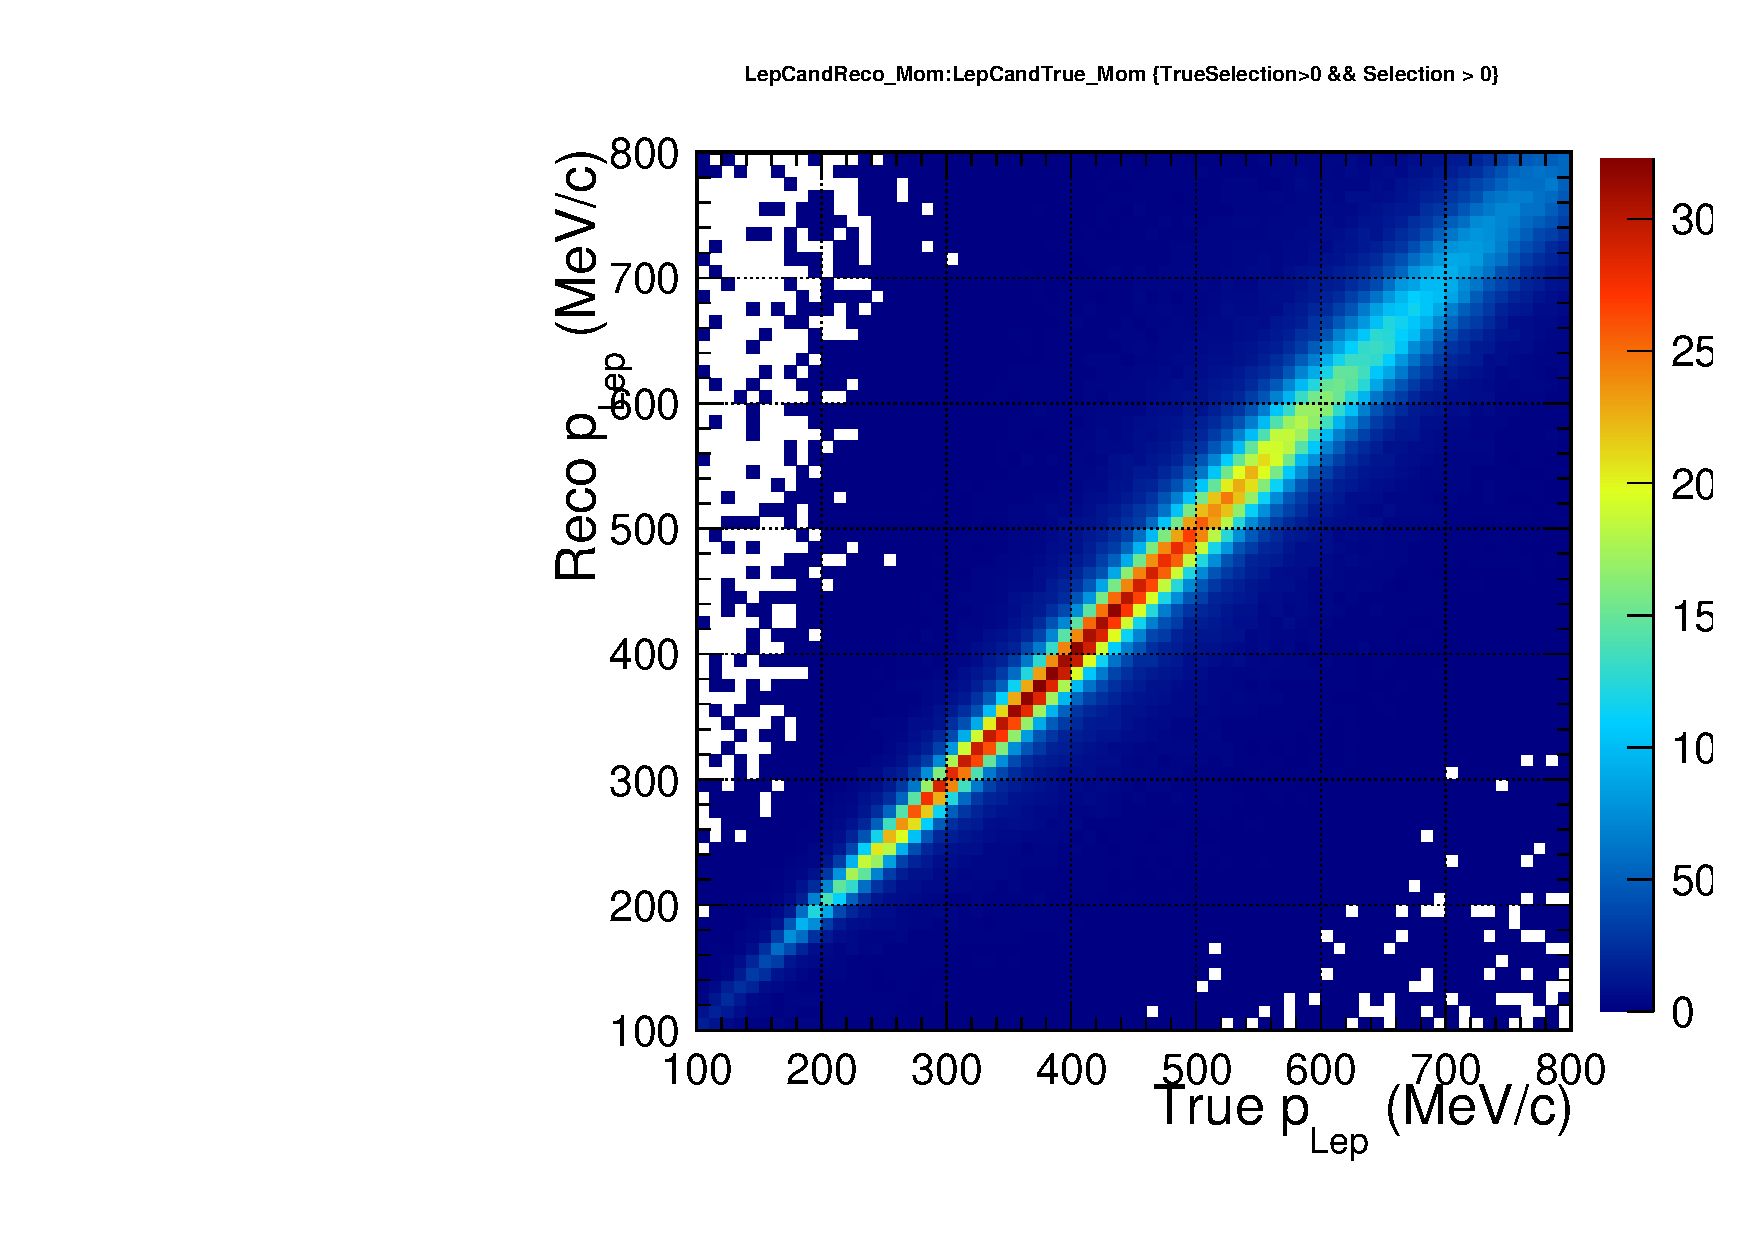
\includegraphics[width=\textwidth, trim={0mm 0mm 0mm 0mm}, clip,page=1]{figures/det/resolution/LepCandTrue_And_Reco_Pmu_ForJacob}
%		\caption{True and reconstructed $p_{Lep}$}
%	\end{subfigure}
	\begin{subfigure}[t]{0.49\textwidth}
		\includegraphics[width=\textwidth, trim={0mm 0mm 17mm 0mm}, clip,page=2]{figures/det/resolution/LepCandTrue_And_Reco_Pmu_ForJacob}
		\caption{Arithmetic mean and RMS}
	\end{subfigure}
	\begin{subfigure}[t]{0.49\textwidth}
	\includegraphics[width=\textwidth, trim={0mm 0mm 17mm 0mm}, clip,page=4]{figures/det/resolution/LepCandTrue_And_Reco_Pmu_ForJacob}
	\caption{RMS}
	\end{subfigure}
	\caption{ND280 momentum resolution for CC-inclusive event's lepton candidates}
	\label{fig:detector_resolution_pmu}
\end{figure}

\autoref{fig:detector_resolution_thetamu} shows the $\theta_{Lep}$ resolution of ND280 for selected events. The resolution is largely flat between $\theta_{Lep}=0-30\text{\degree}$ at 1.5\degree, which linearly increases up to 3\degree at $\theta_{Lep}=70\text{\degree}$. Higher angles are poorly reconstructed ($\Delta \theta_{Lep}=6-25\text{\degree}$) due to the FGD bar orientation, and returns to 7\degree below $\theta_{Lep}=140\text{\degree}$.
\begin{figure}[h]
%	\begin{subfigure}[t]{0.32\textwidth}
%		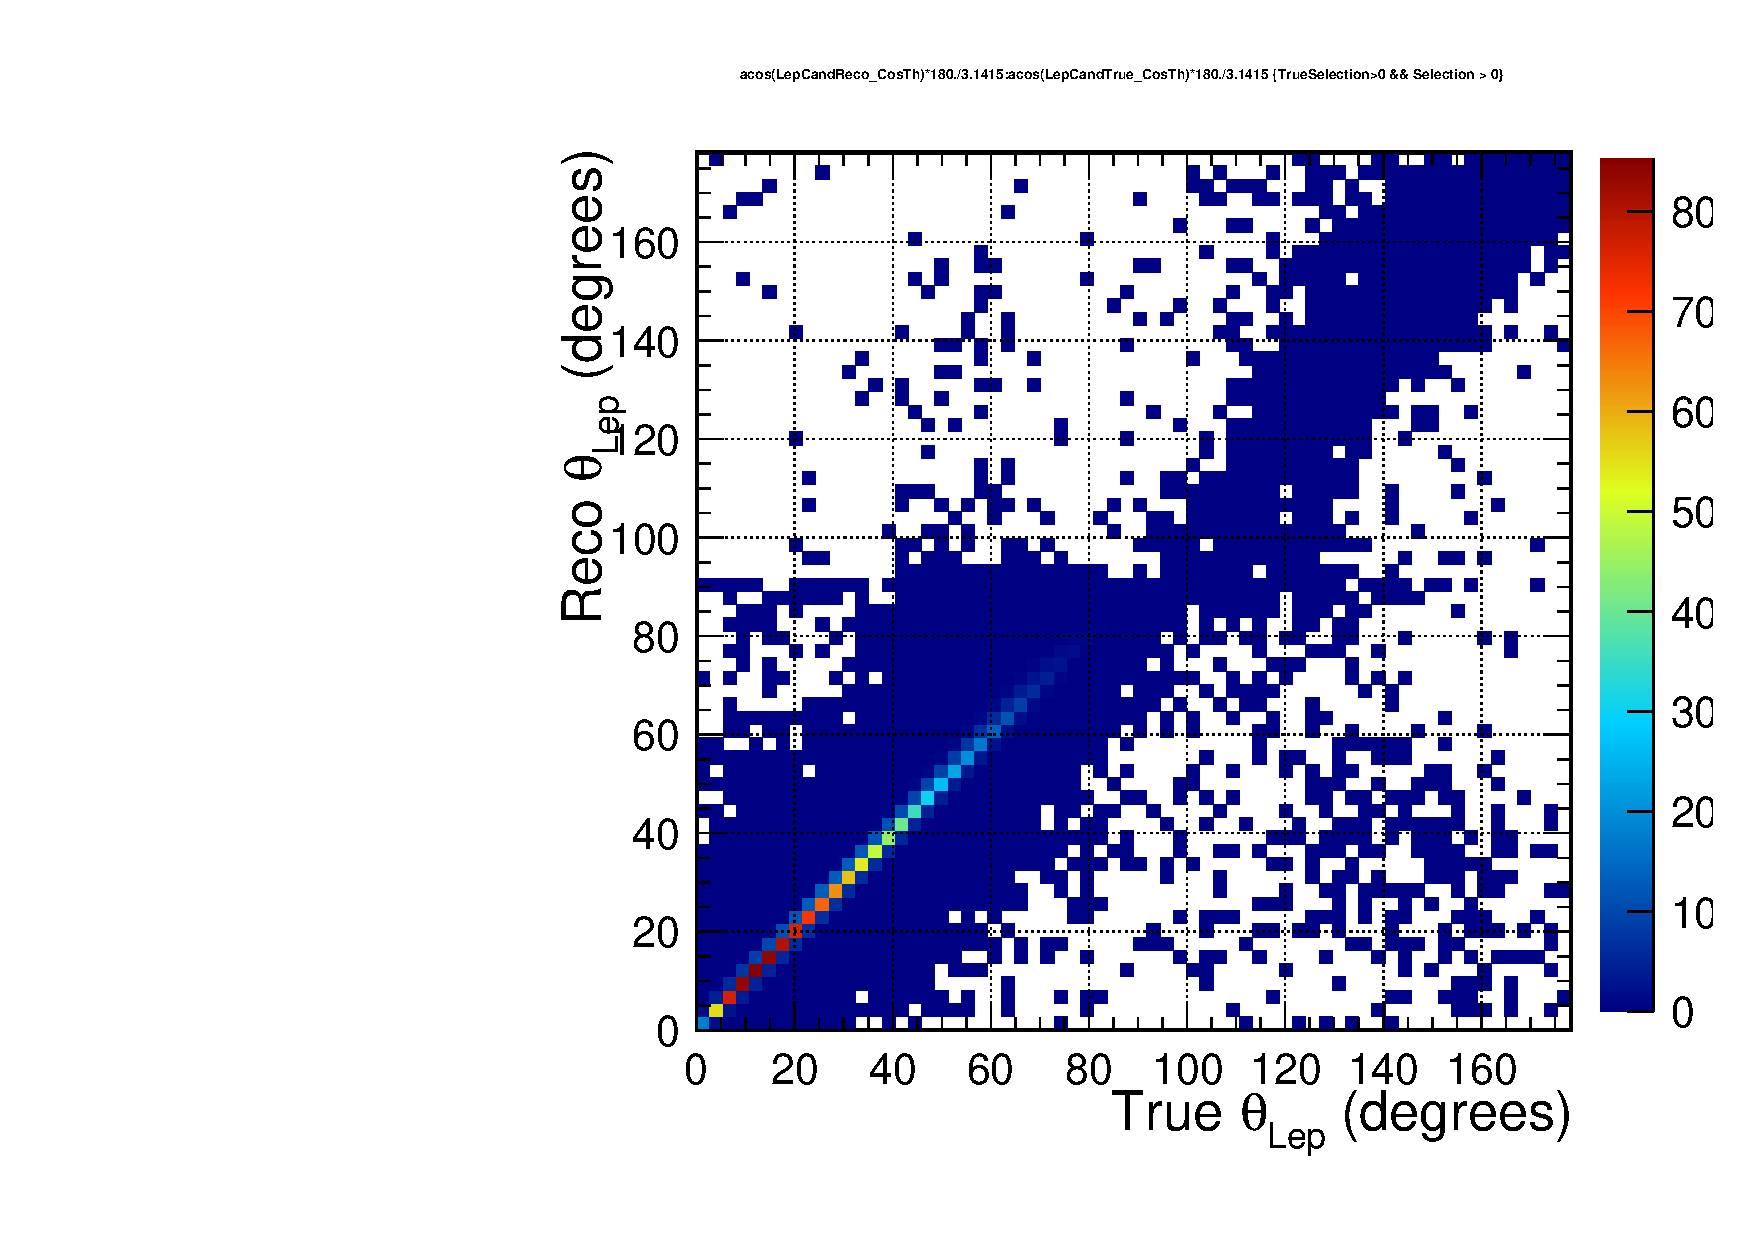
\includegraphics[width=\textwidth, trim={0mm 0mm 0mm 0mm}, clip,page=1]{figures/det/resolution/LepCandTrue_And_Reco_Th_FullRange_ForJacob}
%		\caption{True and reconstructed $\theta_{Lep}$}
%	\end{subfigure}
	\begin{subfigure}[t]{0.49\textwidth}
		\includegraphics[width=\textwidth, trim={0mm 0mm 17mm 0mm}, clip,page=2]{figures/det/resolution/LepCandTrue_And_Reco_Th_Forward_ForJacob}
		\caption{Arithmetic mean and RMS, forward-going}
	\end{subfigure}
	\begin{subfigure}[t]{0.49\textwidth}
		\includegraphics[width=\textwidth, trim={0mm 0mm 17mm 0mm}, clip,page=4]{figures/det/resolution/LepCandTrue_And_Reco_Th_Forward_ForJacob}
		\caption{RMS, forward-going}
	\end{subfigure}

\begin{subfigure}[t]{0.49\textwidth}
	\includegraphics[width=\textwidth, trim={0mm 0mm 17mm 0mm}, clip,page=2]{figures/det/resolution/LepCandTrue_And_Reco_Th_backward_ForJacob}
	\caption{Arithmetic mean and RMS, backward-going}
\end{subfigure}
\begin{subfigure}[t]{0.49\textwidth}
	\includegraphics[width=\textwidth, trim={0mm 0mm 17mm 0mm}, clip,page=4]{figures/det/resolution/LepCandTrue_And_Reco_Th_backward_ForJacob}
	\caption{RMS, backward-going}
\end{subfigure}
	\caption{ND280 $\theta_{Lep}$ resolution for CC-inclusive event's lepton candidates for forward-going (upper panel) and downward-going (lower panel)}
	\label{fig:detector_resolution_thetamu}
\end{figure}